\documentclass[12pt]{article}
\usepackage{graphicx}
\usepackage{hyperref}
\usepackage[a4paper, margin=1in]{geometry}
\usepackage[T1]{fontenc}
\usepackage[utf8]{inputenc}
\usepackage{lmodern}
\usepackage[english]{babel}
\usepackage{xcolor}
\usepackage{pgf,tikz}
%\usetikzlibrary{calc}
\usepackage{amssymb,amsmath,array,bm}
\usepackage[T1]{fontenc}
\usepackage[utf8]{inputenc}
\usepackage{hyperref}
\usepackage{multicol}
\usepackage{tabularx}

\hypersetup{
	colorlinks,
	linkcolor={black},
	citecolor={black},
	urlcolor={black}
}

\newcommand{\titleGP}{\begingroup
	\centering
	\vspace{\baselineskip}
	
	\rule{\textwidth}{1.6pt}\vspace{-\baselineskip}\vspace{2pt}
	\rule{\textwidth}{0.4pt}\\[\baselineskip]
	
	{\LARGE Math Expressions Calculator}\\[0.2\baselineskip]
	
	\rule{\textwidth}{0.4pt}\vspace{-\baselineskip}\vspace{3.2pt}
	\rule{\textwidth}{1.6pt}\\[\baselineskip] % Thick horizontal line
	
	
\includegraphics[scale=0.5]{logo2.png}
	\\
	
	\vspace{50pt}
	{\LARGE Alex Ivanov Tsvetanov\\\par}
	{\itshape \Large Sofia High School of Mathematics \\ Sofia, Bulgaria\par}
	
	\vspace{2\baselineskip}
	
	{\scshape \large
	Under the direction of \\
	ch. ace. Emil Kelevedjiev \\\par
	}
	\vspace{1cm}
	
	
	\vfill
	
	{\scshape 2016} \\[0.3\baselineskip]
	{\large SRS, Blagoevgrag, Bulgaria }\par
	
	\endgroup}

\begin{document} 
	
	\pagestyle{empty}
	
	\titleGP
	\newpage
	\tableofcontents
	\newpage

\begin{center}\LARGE \textbf{Summary}\end{center}
There are many tools for performing calculations and data processing (like wolframalpha.com and MS Excel) but they cannot allow you to create custom new operations (functions, brackets, etc.).
That is why our program is better than them.
This project aims at making an application, which calculates and simplifies expressions with custom data types. It is different than the other tools because it provides an option for run-time addition of custom operations, variables, arrays, pairs of brackets and functions. It can be used for scientific and learning purposes.

\section{Introduction}
This application improves the work with databases and big data, because it makes the code easier to read. This is useful for both scientists and young students, because it can help them with suggestions for better solutions by checking their answers. \\
We have implemented expression calculation with an option for run-time addition of operations, variables, pairs of brackets, functions and find derivative functions.

\section{Implementation}
	\subsection{Structuring}
	For the structuring we use Object-Orientated Programming(OOP) with C++. \\ \\
	{\small
	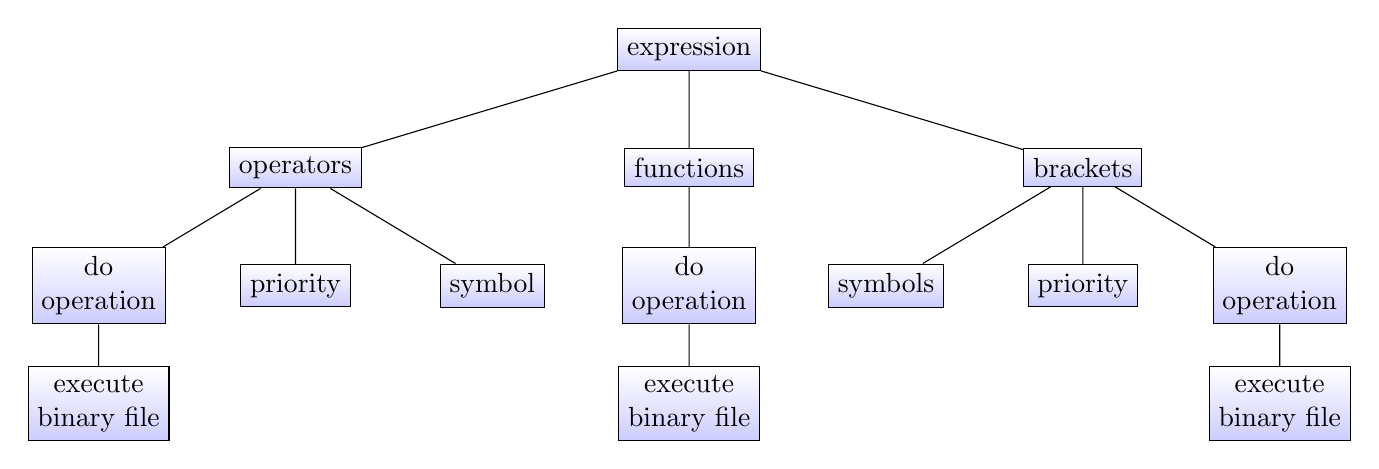
\begin{tikzpicture}[
	auto,
	level 1/.style={sibling distance=50mm},
	level 2/.style={sibling distance=25mm},
	level 3/.style={sibling distance=10mm},
	every node/.style = {shape=rectangle,
		draw, align=center,
		top color=white, bottom color=blue!20}]
	\node[draw] {expression}
	child
	{
		node[draw] {operators}
		child
		{
			node[draw] {do\\operation}
			child
			{
				node[draw] {execute \\ binary file}	
			}
		}
		child
		{
			node[draw] {priority}	
		}
		child
		{
			node[draw] {symbol}	
		}
	}
	child
	{
		node[draw] {functions}
		child
		{
			node[draw] {do\\operation}
			child
			{
				node[draw] {execute \\ binary file}	
			}	
		}
	}
	child
	{
		node[draw] {brackets}
		child
		{
			node[draw] {symbols}	
		}
		child
		{
			node[draw] {priority}	
		}
		child
		{
			node[draw] {do\\operation}	
			child
			{
				node[draw] {execute \\ binary file}	
			}
		}
	}
	;
	\end{tikzpicture}
	}
	\subsection{Graphical view}
	For the graphical view we use HTML and MathJax.\\ \\
	{\small
		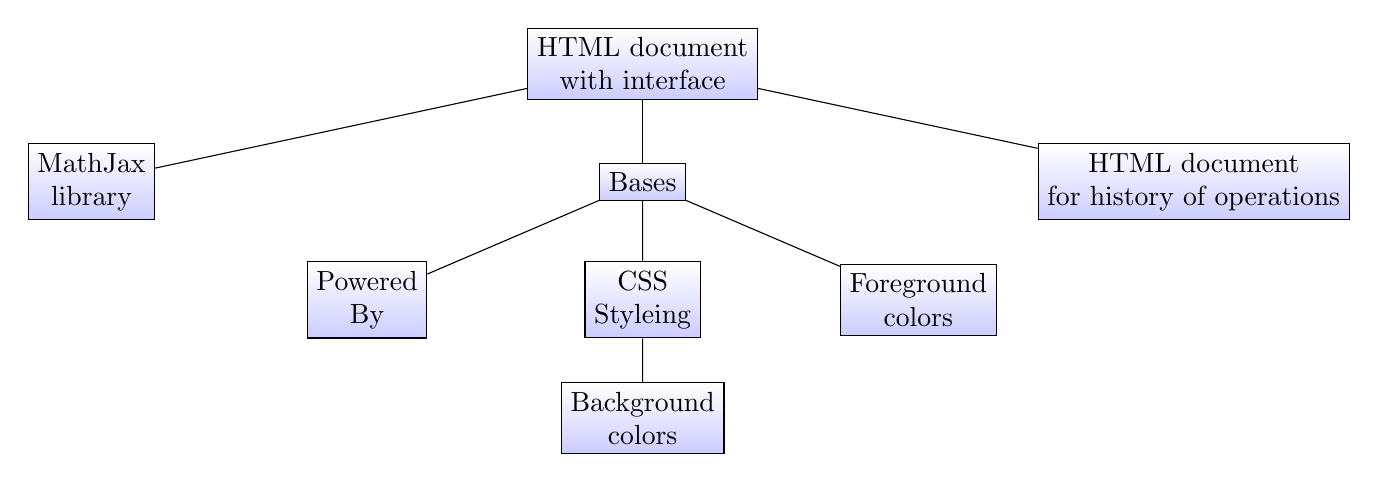
\begin{tikzpicture}[
		auto,
		level 1/.style={sibling distance=70mm},
		level 2/.style={sibling distance=35mm},
		level 3/.style={sibling distance=17mm},
		every node/.style = {shape=rectangle,
			draw, align=center,
			top color=white, bottom color=blue!20}]
		\node[draw] {HTML document\\with interface}
		child
		{
			node[draw] {MathJax\\library}
		}
		child
		{
			node[draw] {Bases}
			child
			{
				node[draw] {Powered\\By}	
			}
			child
			{
				node[draw] {CSS\\Styleing}
				child
				{
					node[draw] {Background\\colors}	
				}
			}
			child
			{
				node[draw] {Foreground\\colors}	
			}
		}
		child
		{
			node[draw] {HTML document\\for history of operations}
		}
		;
		\end{tikzpicture}
	}
%	\subsection{Parsers}
%	For the parsers we use C++ and our script language syntax.
\section{Functions of application}
{\Large In the following table are described the functions of our program:}
\begin{table}[ht]
	\centering
	\resizebox{\textwidth}{!}{\begin{tabular}{c|c|c}
			Function & Description & Example\\
			\hline
			No/End   & Each of the execution  & End\\
			\hline
			I want more!   & Adds new functions &  \\
			\hline
			(...)'   & Gives you the derivative function &  (a+b)' \\
			\hline
			calc   & Calculates the expression & calc (a+b)*c \\
			\hline
			set   & Sets value of a variable & set d (a+b)*c \\
			\hline
		\end{tabular}}
	\end{table}
		\section{Technologies}
		To implement the software we use C++ for better performance (speed and memory) and easier structuring of the OOP part. We make the graphical preview using HTML and JavaScript (MathJax). For the run-time addition we downgrade the math script to C++ and compile it with GNU Compiler Collection (GCC). \\
		{\centering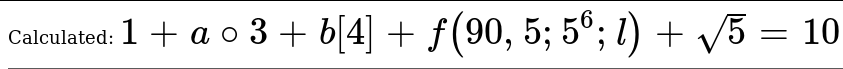
\includegraphics[scale=0.5]{screeenshot_SRS.png}}
		\section{Future work}
		This project provides space for future improvement. We will work further on the interface and the functionality(by adding case defined functions and others). This is something like:\\
		\[
		  f (expr) = \left\{\begin{array}{ll}
		  f (a) + f (b), & \text{for } expr = a + b\\
		  0, & \text{for } expr = const\\
		  b * a ^ {b - 1}, & \text{for } expr = a ^ b\\
		  ... & ...
		  \end{array} \right.
		\]
		{\begin{center} Ex.1: \textbf{\textit{derivative function}}\end{center}}
		\section{Conclusion}
		This project helps working with big data and databases by making the code more human readable. This is useful for both scientists and young students, because it can help them by checking their answers and suggesting them better solutions. \\
		In the future this project will include arrays and integral calculation. It will be modified so that it could be used as an open-source library. \\
		\section{Acknowledgments}
		Special thanks to:
		\begin{itemize}
			\item Konstantin Simeonov and Pano Panov for the idea
			\item Emil Kelevejiev for the improvement of the project
			\item Todor Branzov for the help with the management of this project
			\item Konstantin Delchev for the help with the base questions
			\item Kristian Georgiev
		\end{itemize}
		Thanks also to:
		\begin{itemize}
			\item High School Students Institute of Mathematics and Informatics
			\item Bulgarian Academy of Sciences
			\item Sofia High School of Mathematics
			\item Telerik a Progress Company
		\end{itemize}
		\begin{thebibliography}{99}
	
		\bibitem{gcc}
		{\itshape GNU Compiler Collection}.
		\texttt{https://gcc.gnu.org/}. \\
		Copyright \copyright\; 2009 Free Software Foundation, Inc.
		\bibitem{mathjax}
		{\itshape MathJax}.
		\texttt{https://www.mathjax.org/}. \\
		Copyright \copyright\; 2015 The MathJax Consortium.
		\bibitem{latex}
		{\itshape \LaTeX}.
		\texttt{https://www.latex-project.org/}.
		\end{thebibliography}
		
	\end{document}